\chapter*{Pares de elementos}
\addcontentsline{toc}{section}{Pares de elementos}
\markboth{Pares de elementos}{Pares de elementos}

En muchos problemas nos pedirán que encontremos o contemos la cantidad de pares que cumplan alguna condición, o nosotros convertiremos a un problema de este estilo. Para este tipo de problemas será útil conocer como hacer una búsqueda completa que revise todas las posibles parejas de elementos.

Como antes, veamos un problema que puede ser resuelto con esto.

\section*{Ejemplo 2.1.1}
\addcontentsline{toc}{subsection}{Ejemplo 2.1.1}

Fernando necesita \(K\) tornillos de la ferretería. Sin embargo, la vida no siempre es fácil y la ferretería no vende exactamente \(K\) tornillos.

Sin embargo, venden \(N\) cajas de tornillos cada una con \(C_i\) tornillos dentro. 

Como Fernando tiene una obsesión con no desperdiciar, él solo comprara las cajas de forma que traigan juntas exactamente \(K\) tornillos. Además, odia las bolsas de un solo uso que dan en la ferretería por lo que solo comprará dos cajas, una por cada mano.

Entonces, dado el tamaño de las cajas, determina si Fernando puede traer consigo exactamente \(K\) tornillos.

\subsection*{Entrada}
Dos enteros, \(N\) y \(K\), representando cuantas cajas hay y cuantos tornillos se requieren.

En la siguiente línea vendrán \(N\) enteros separados por espacios, indicando la cantidad de tornillos en cada caja.

\subsection*{Salida}
Deberás imprimir “SI” en caso de que Fernando pueda obtener K tornillos con sus reglas, o “NO” si es imposible.

\subsection*{Casos ejemplo}

\begin{casebox3}
	\ecase{
		4 6 \\
		3 1 8 5
	}
	{SI}
	{Usa las cajas con 1 y 5 tornillos.}
	\ecase{
		5 10\\
		3 1 8 5 12
	}
	{NO}
	{}
\end{casebox3}

\subsection*{Límites}
\begin{plimits}
	\item \(1\leq N \leq 1000\)
	\item \(1\leq K \leq 10^9\)
	\item \(1\leq C_i \leq 10^9\)
	\item \(C_i \neq K\)
\end{plimits}

Enlace: [TODO]

\section * {Solución}

Lo que nos pregunta el problema es: ¿Existe un par de cajas tal qué sumen \(K\)?

Para determinar si existe dicha pareja, lo que haremos será buscar entre todas las parejas de cajas aquella que sume \(K\). Es decir, buscaremos completamente todas las parejas posibles.

Para iterar por todas las parejas lo que haremos es primero definir una pareja como dos índices \((i,j)\), tal que \(0\leq i < j <N\).  Como queremos iterar por todos los posibles pares, primero iteraremos por todos los valores de \(i\). Y para cada \(i\), iteraremos por todas las \(j\) con las que se puede emparejar. El código se ve como:

\begin{lstlisting}
for (int i =0; i < N; i++) {
	for (int j=i+1; j< N; j++) {
		cout << i<<" "<<j<< "\n";/* imprimimos 
		cada par */ 
	}
}
\end{lstlisting}

Y ahora que sabemos iterar por todos los pares, lo utilizamos para revisar si existe un par que sume \(K\). 

\begin{lstlisting}
for (int i =0; i < N; i++) {
	for (int j=i+1; j< N; j++) {
		if (Caja[i]+Caja[j] == K) {
			cout << "SI";
			exit(0); /* Termina el programa, 
			encontramos la respuesta */
		}
	}
}
cout << "NO";
\end{lstlisting}

Entonces, son estos dos ciclos for nos permiten iterar por toda pareja de elementos en un arreglo. Esta es una herramienta bastante útil para resolver muchos problemas y subtareas.

\section * {Complejidad}
\addcontentsline{toc}{subsection}{Complejidad}
Bien, ahora hablemos de la complejidad de esta técnica. La complejidad es \(O(N^2)\). Esto es porque la cantidad de parejas con \(N\) elementos crece en\(O(N^2)\).

Pero incluso si no conocemos como crecen las parejas, podemos ver que este ciclo para \(i = 0\), itera por \(N-1\) valores de \(j\); para \(i=1\), iteramos por \(N-2\) valores de \(j\); para \(i=2\), iteramos por \(N-3\) valores de \(j\), y así sucesivamente. De forma que hacemos \((N-1)+(N-2)+\ldots+1+0\) iteraciones de \(j\). Entonces hacemos \(1+2+3+\ldots+(N-1)\) iteraciones.

Usando la formula se suma de gauss\footnote{Formula de gauss para sumar los primeros \(N\) naturales: \(1+2+3+\ldots+N=\frac{N(N+1)}{2}\)} obtenemos que:

\[1+2+3+\ldots+(N-1)=\frac{N(N-1)}{2}=\frac{N^2}{2}-\frac{N}{2}\]

Entonces, la complejidad queda como \(O(\frac{N^2}{2}-\frac{N}{2})=O(N^2)\)

Por lo tanto, iterar por todos los pares de un arreglo es una técnica de complejidad cuadrada, perfecta para límites hasta \(\sim{10^4}\).

\newpage

\practiceproblemsection{2.1}

\problemtitle Definimos una inversión como una parejas \((i,j)\) en un arreglo tal que \(1\leq i < j \leq N\) y también \(A_i > A_j\). Es decir, una pareja de números que estén al revés de como deberían estarlo en un orden de menor a mayor.

Dado un arreglo de \(N\) enteros, imprime cuantas inversiones hay en él.

\subsubsection*{Ejemplo}
\begin{casebox3}
	\ecase{
		4\\
		3 2 6 1
	}
	{4}
	{
		Las inversiones son: \\
		El 3 con el 2, \\
		el 3 con el 1,\\
		el 2 con el 1, \\
		y el 6 con el 1. 
	}	
\end{casebox3}
\subsubsection*{Límites}
\begin{plimits}
	\item \(1\leq N \leq 5000\)
	\item \(1\leq A_i \leq 10^9\)
\end{plimits}

Enlace: [TODO]

\problembreak

\problemtitle Fernando regreso el otro día a la tienda de tornillos, y esta vez quiere darle una puntuación en un sitio web de guías locales. Fernando juzga la calidad de la tienda en función de cuantas cantidades diferentes de tornillos él puede comprar.

Recordemos que la tienda vende \(N\) cajas de tornillos, cada una con \(C_i\) dentro. Recordemos que Fernando solo puede tomar una o dos cajas en una compra porque solo tiene dos manos.

Dado las cajas de tornillos, determina la calidad de la tienda.

\subsubsection{Ejemplo}
\begin{casebox3}
	\ecase{
		3\\
		1 3 4
	} 
	{5}
	{
	   Fer puede hacer compras de \\
	   1, 3, 4, 5 o 7 tornillos.
	}
\end{casebox3}

\subsubsection*{Límites}
\begin{plimits}
	\item \(1\leq N \leq 10^5\)
	\item \(1\leq A_i \leq 10^3\)
\end{plimits}

Enlace: [TODO]

\problembreak

\problemtitle La revista “algofashion” dijo esta semana que los números a la moda son aquellos que pueden ser representados como la suma de dos números pertenecientes a la secuencia de Fibonacci.

Recordemos que la secuencia de Fibonacci empieza con dos 1. Y luego cada número será resultado de la suma de los dos anteriores.
\[F_1=F_2=1\]
\[F_n=F_{n-1}+F_{n-2}\]

De forma que los primeros números de la secuencia son:
 \[1,1,2,3,5,8,13,21\ldots\]

Karel acaba de leer la revista y ahora quiere responder \(T\) preguntas, cada pregunta será del tipo: ¿El número \(x_i\) está de moda?

Como amigo, debes hacer un código que responda las dudas de Karel.

\subsubsection*{Entrada}
En la primera línea vendrá el valor de \(T\), cuantas preguntas tiene Karel.

En las siguientes \(T\) líneas vendrán las preguntas de Karel, una por línea. Cada pregunta consiste en un solo entero \(x_i\).

\subsubsection*{Salida}
Imprime \(T\) líneas, cada una siendo la respuesta a una pregunta de Karel. La línea \(i\) debe ser “SI” si \(x_i\) está a la moda y debe ser “NO” si no está a la moda. 

\subsubsection*{Caso ejemplo}	

\begin{casebox2}
	\scase{
		3\\
		5\\
		6\\
		10
	}
	{
		SI\\
		NO\\
		SI
	}
\end{casebox2}

\subsubsection*{Límites}

\begin{itemize}
	\setlength{\parskip}{1pt}	
	\item \(1\leq T \leq 100\)
	\item \(1\leq x_i \leq 10^{18}\)
\end{itemize}

Enlace: [TODO]

\problembreak

\problemtitle Tú tiene una constructora que busca comprar un terreno para construir un fraccionamiento.

Actualmente, el gobierno de Karelopolis permite que compres un terreno en la región para desarrollo. La región para desarrollo se ve como una cuadricula de \(N\) filas y \(M\) columnas. El terreno que compres debe ser rectangular y alineada a la cuadricula, es decir, no puedes comprar una celda de la cuadricula de forma incompleta.

Además, tu calculaste cuanto dinero obtendrías si compras cada celda, en concreto, la celda que esta en la fila \(i\) y columna \(j\) aportaría \(v_{ij}\) pesos. Como hay celdas con valor positivo y otras con valor negativo, te preguntas cual es el máximo valor que puedes obtener.

Por ejemplo, si la región para desarrollo se ve de la siguiente forma:

\begin{center}
		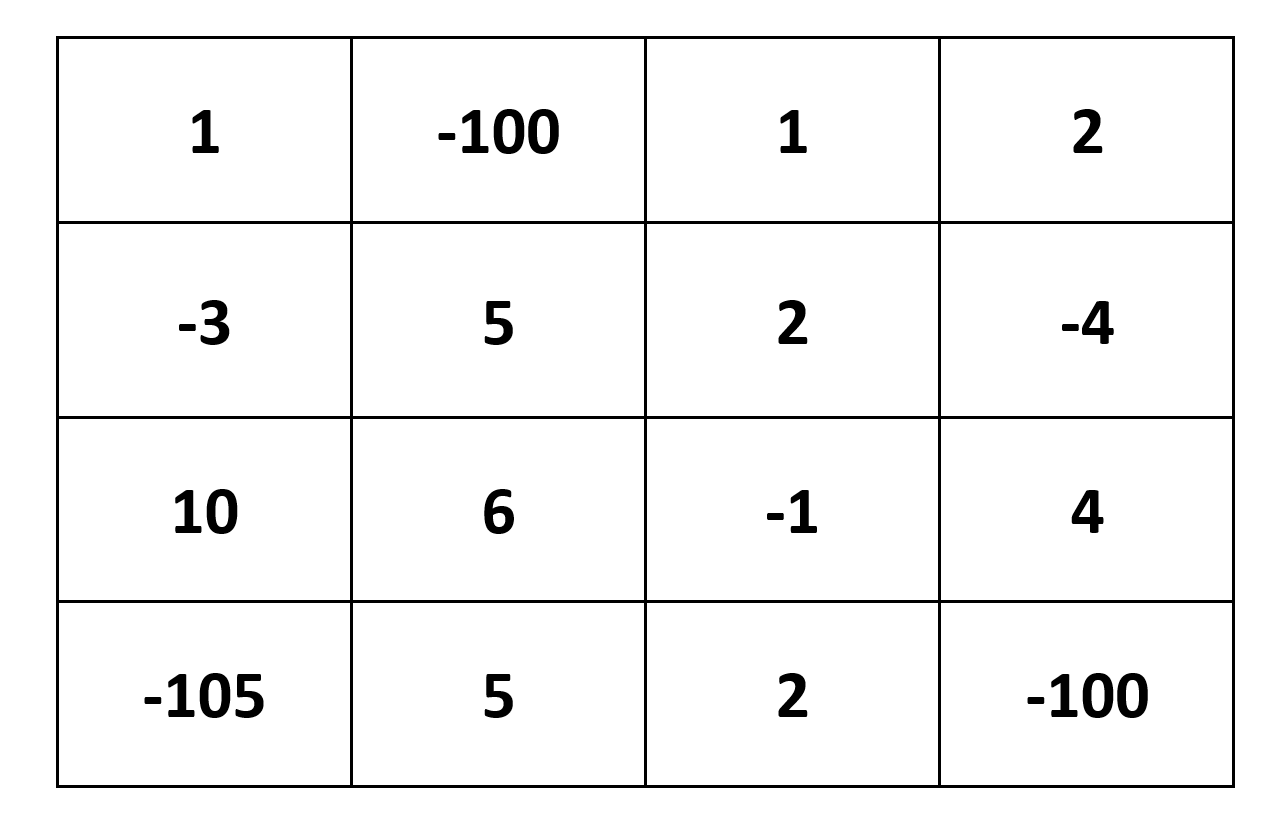
\includegraphics[scale=0.15]{terrenos}
\end{center}

Tu puedes obtener hasta 19 pesos comprando el terreno:

\begin{center}
	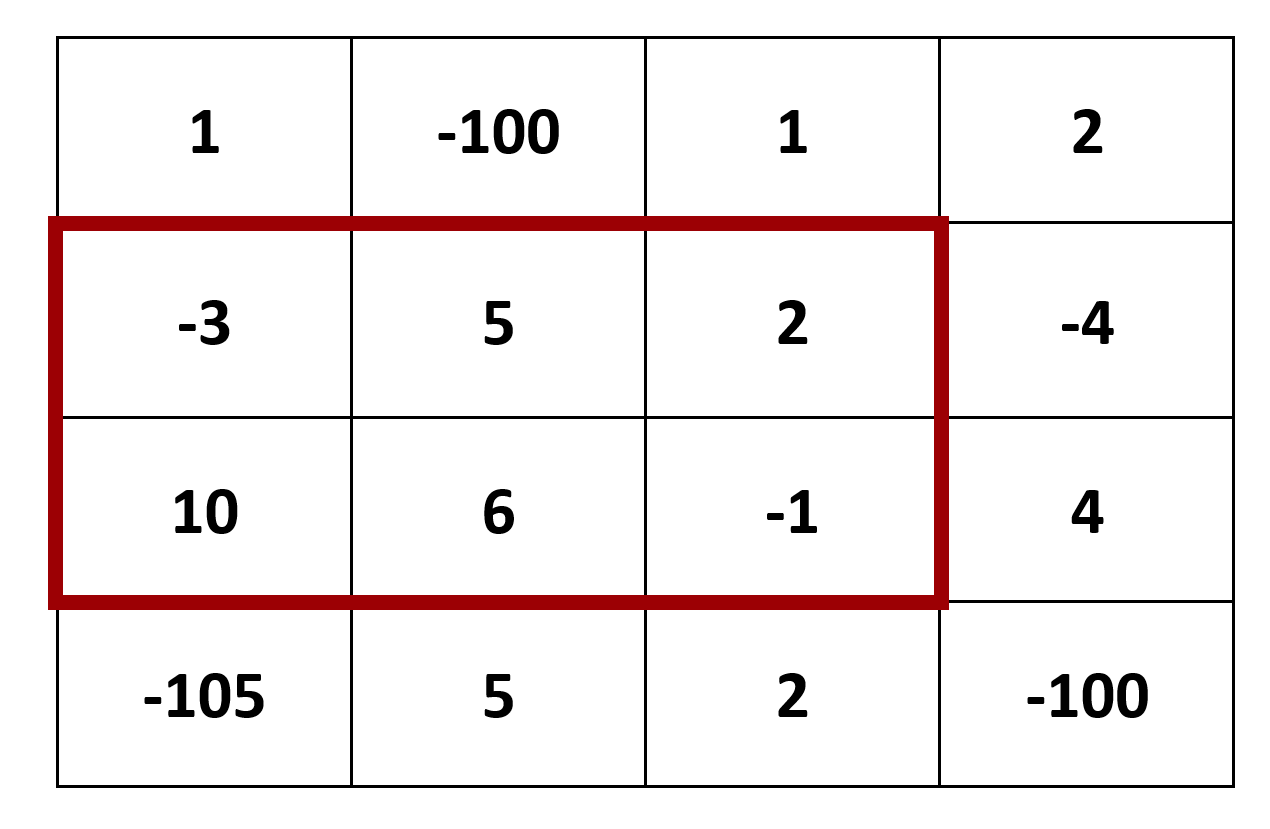
\includegraphics[scale=0.15]{terrenos2}
\end{center}


Encuentra el máximo valor posible si compras un terreno dada la región para desarrollo.

\subsubsection*{Entrada}

En la primera línea recibes \(N\) y \(M\).

En las siguientes \(N\) líneas recibirás \(M\) enteros representando los valores de \(v_{ij}\).

\subsubsection*{Salida}

Un entero que sea el mayor valor de un terreno.

\subsubsection*{Ejemplo}

\begin{casebox2}
	\scase{
		4 4\\
		1 -100 1 2\\
		-3 5 2 -4\\
		10 6 -1 4\\
		-105 5 2 -100
	}{19}
	\hline
\end{casebox2}

\subsubsection*{Límites}

\begin{plimits}
	\item \(1\leq N, M\leq 75 \)
	\item \(-10^9\leq v_{ij}\leq 10^9 \)
\end{plimits}

\subsubsection*{Subtareas}

\begin{plimits}
	\item (40 pts) \(1\leq N, M\leq 15 \)
	\item (60 pts) Sin consideraciones extra.
\end{plimits}

Enlace: [TODO]

\problembreak

\problemtitle Dado un arreglo \(A\) de \(N\) enteros. Determina si existe un par de elementos que su suma modulo \(P\) sea \(K\) .

\subsubsection*{Límites}
\begin{plimits}
	\item \(1\leq N,K,P\leq 10^5 \)
	\item \(1\leq A_i\leq 10^9 \)
\end{plimits}

\subsubsection*{Subtareas}
\begin{plimits}
	\item (25 puntos) \(1\leq N\leq 10^3 \)
	\item (50 puntos) \(1\leq K, P\leq 10^3 \)
	\item (25 puntos) Sin restricciones extra.
\end{plimits}

Enlace: [TODO]